% vim: set ts=2 sw=2 noet spell:

\chapter{Implementation}

\section{Overview}

% TODO: quelle https://wiki.gnuradio.org/
For the simulation task and after for the Hardware part, the open-source Software GNU Radio has been chosen. This software uses toolboxes for signal processing systems too simulate or/and implement a software-defined radio, based on Python and some C++ implementations for some rapid-application-development environments. The toolboxes can simply, with the help of the graphical user interface, used by drag-and-drop. The Boxes are used to write applications, to receive or to transmit date for a digital system. Some blocks like different filters, channel codes or demodulator elements and a lot more are already implemented. For missing application new elements can be added by coding own blocks. With the help of the GNU Radio software those toolboxes can easily get connected to each other, creating data streams. 

\section{Sender chain}
\subsection{Data frame}

\begin{figure}
	\centering
	% vim:ts=2 sw=2:
\begin{tikzpicture}[
		brace/.style = {
			decorate,
			decoration = {
				calligraphic brace,
				amplitude = 3mm,
				raise = 1mm,
				mirror,
			},
			very thick,
			pen colour = {black} 
		},
	]
	\matrix[
		column sep = -1pt,
		nodes = {
			draw, rectangle, very thick,
			minimum height = 12mm,
			text width = 20mm,
			align = center,
		},
	]{
		\node[] {Preamble \\ \(k\) Bytes}; &
		\node[fill=lightgray!20] (pad) {Padding \\ 1 Bit}; &
		\node[fill=red!10] (id) {ID \\ 5 Bits}; &
		\node[fill=red!10] {Length \\ 21 Bits}; &
		\node[fill=red!10] (par) {Parity \\ 5 Bits}; &
		\node[] {Payload \\ \(\ell\) Bytes}; \\
		% \node{Padding }; \\
	};

	\draw[brace] (id.south west) --
		node[midway, below = 5mm] {(31, 26) Hamming ECC}
		(par.south east);

	% \draw[brace] (par.north east) --
	% 	node[midway, above = 5mm] {4 Bytes}
	% 	(pad.north west);

\end{tikzpicture}

	\caption{
		Structure of framed data packets used in the implementation.
		\label{fig:dataframe}
	}
\end{figure}

To compute the empirical \emph{bit error rate} (BER) of the setup, the data has to be framed on by the sender and the bitstream synchronized on the receiver side. The structure of a data packed used in the implementation is shown in \figref{fig:dataframe}. A frame begins with an user specified \(k\)-byte preamble, that in the current implementation serves as synchronization pattern. Another use case for the preamble sequence could be to introduce channel estimation pilot symbols. Following the preamble are 4 bytes encoded using a (31, 26) Hamming code (plus 1 padding bit), that contain metadata about the packet, namely payload ID and payload length. Because the payload length in bytes is encoded in 21 bits, the maximum payload size is 2 MiB, which together with 32 possible unique IDs gives a maximum data transfer with unique frame headers of 64 MiB. These constraints are a result of decisions made to keep the implementation simple.


\subsection{Modulation}

The constellation modulator block is used for a root-raised-cosine-filtered basis modulation. The block gives an input of a byte stream as complex modulated signal in the baseband back. 
Further more it's possible to chose the modulation type here, in this example it is 16QAM, but QPSK, 8PSK and BPSK would also be possible.

\section{Receiver chain}

\subsection{Envelope detector}

\paragraph{Polyphase Clock Sync}
%% To Do : nochmals anschauen ob dieese erklärung verständlich ist und richtig interpretiert wurde.
With the the polyphase clock sync the symbols can be synchronized by preforming a time synchronization with the help of multiple filterbanks. For that the derivation of the filtered signal should be minimized whish turns to a better SNR. This works with the help of two filterbanks, one of them contains the filters of the signal adapted to the pulse shaping with several phases. The other contains its derivative. So in the time domain it has a sinc shape, for the output Signal the sinc peak should be on a sample, with the fact that sinc(0) = 1 and sinc(0)' = 0 an error signal can be generated which tells how far away from the peak it is. This error Signal should be zero this is possible with the help of a loop second order whish constants the number of the filterbank and the rate. This rate is generated because of the clock difference between the transmitter and reviver to synchronies the receiver the filter goes through the phases. For the output one sample per symbol is enough.

\paragraph{Equalizer}

\skelpar[2]{CMA equalizer.}

\subsection{Frame synchronization and phase correction}

Once the envelope's clock is synchronized in the processing chain the data stream has one sample per symbol. At this point it is necessary to find where each data frame starts or end in order to correctly decode their payloads. For such purpose a special sequence of samples called \emph{access code} is put in front of each frame. Access codes are sequences of samples that are specially chosen to have autocorrelation values with a high peak at zero, and that rapidly descend for other shifted value. In other words, the autocorrelation of an access code high only when the sequence is perfectly aligned. Thus by cross correlating an envelope signal \(r(t)\), that periodically contains an access code \(a(t)\) with the access code itself, and looking for peaks in the result, it is possible to determine where each frames begin. Furthermore by analyzing the values of the peaks it is possible to extract informations about the phase and frequency offsets.

To actually see how that is possible, recall that mathematically the cross correlation (denoted here by \(\star\)) of two values complex signals is
\begin{equation}
	R_{ra}
	= r(t) \star a(t)
	= \int_\mathbb{R} r(\tau) a^*(\tau - t) \,d\tau
	= r(t) * a^*(-t),
\end{equation}
which is equivalent to a convolution, where the left term being time-reversed complex conjugated \cite{Gallager}. This last property is especially useful because it makes possible to implement cross correlation using FIR filters. Some interesting properties of the cross correlation are that correlation with itself (also called autocorrelation) at \(t = 0\) is
\begin{equation}
	R_{aa} = (a \star a)(0)
	= \int_\mathbb{R} a(\tau) a^*(\tau - 0) \,d\tau
	= \int_\mathbb{R} |a(\tau)|^2 \,d\tau \in \mathbb{R},
\end{equation}
which is a real number. And the correlation with an out of phase copy \(a'(t) = a(t) e^{j\varphi}\) is
\begin{equation}
	% R_{a'a} =
	(a' \star a)(0) 
	= \int_\mathbb{R} a(\tau)e^{j\varphi}  a^*(\tau) \,d\tau
	= R_{aa} e^{j\varphi}.
\end{equation}
The important thing to notice in the previous expression is that since \(R_{aa}\) is a real number, the phase of the cross correlation at \(t = 0\) is the phase of \(a'(t)\). This fact is used to implement a fine phase correction for the received envelope in relatively few steps as follows:
\begin{itemize}
	\item Compute the cross correlation of the envelope \(r(t)\) with the access code \(a(t)\), i.e. \(R_{ra}(t) = (r \star a)(t)\).
	\item Find the maximum value of \(\hat{R}_{ra} = \max R_{ra}(t)\) (correlation peak).
	\item Extract the phase offset \(\varphi = \angle \hat{R}_{ra}\).
	\item Remove the phase offset in the envelope by multiplying with the complex conjugate of the offset, that is \(\hat{r}(t) = r(t) e^{-j\varphi}\)
\end{itemize}
%% TODO: frequency correction using linear interpolation

\section{Channel simulations}

Here its possible to add some AWGN noise in the channel line. Different parameters can be changed like the noise voltage, time or the frequency offset.

\skelpar[5]{
	Discuss the multitap FIR model we used. How it is possible to set the delay etc. Also mathematics for the interpolation.
}

%To get a basic line for further simulations a 16QAM has been made. The results of this simulation are shown in \figref{fig:simul16QAM} and \figref{fig:simul16QAM_1} as the red Signal. In \tabref{tab:modulation_settings} some importer Parameter settings for a different modulation scheme are mentioned.
%
%A FIR-Filter was added in the Channel to create a time delay between tow paths. In \figref{fig:simul16QAM} the result includes a direct path and a delayed one. In the plot of \figref{fig:simul16QAM_1} the transmission line dosn't include a direct path. %It's impotent to mention that the delay should be smaller than the symbol rate or a multiple of it. (Stimmt dies , not sure any more)
%
%For the a first simulation with some fading the 16QAM simulation model has been extended with a FIR-Filter in the Chanel. The results of this simulation are shown in \figref{fig:simul16QAM} and \figref{fig:simul16QAM_1} as the blue Signal.

\subsection{Fading}
%TO DO: übersetzen 
Für die statische implementation und veranschaulichen des Fading effekts wurde ein eigener Block kreaiert und in den Channel implementiert. Dieser Block basiert auf einem FIR Filter. Es kann mit direcktem Pfad oder ohne dargestellt werden (Line of Side). Mit Hilfe dieses Filters wird die Verspätung der nebenpfaden dargestellt. Es ist möglich beliebig viele dieser Pfade mit unterschiedlicher stärke zu simulieren. Dieser Block wurde zusätzlich mit der methode in \ref{sec:fractional-delay} beschriben implementiert um nichtganzahlige delay werte zu erlauben.

% Bild einfügen 





\section{Hardware}

As Hardware we chosen the USRP B210 from Ettus Research, with the following specifications shown in \tabref{tab:USRP B210 specifications}. Because this SDR is more than enough for our requires.

For the Hardware setup up some changes are made in the file from the 16QAM simulation to fit with the SDRs. For the first test a coaxial cable was used as transmission line, after the cabel were been replaced with two antennas. The gnu radio block scheme is shown in \figref{fig:simul16QAM_Hardware_Aufbau}. The results for s anntena set uo with a transmission line of 20cm  are plotted in \figref{fig:simul16QAM__Hardware}.

Instead of the channel modeling block the USRP blocks are used. The sink as transmitter and the source as resiver.  The Signal is sended on a center frequency of 2.4GHz.

\subsection{Empirical BER} \label{sec:ber}

\subsection{Measurements}

%
%
%

\begin{figure}
	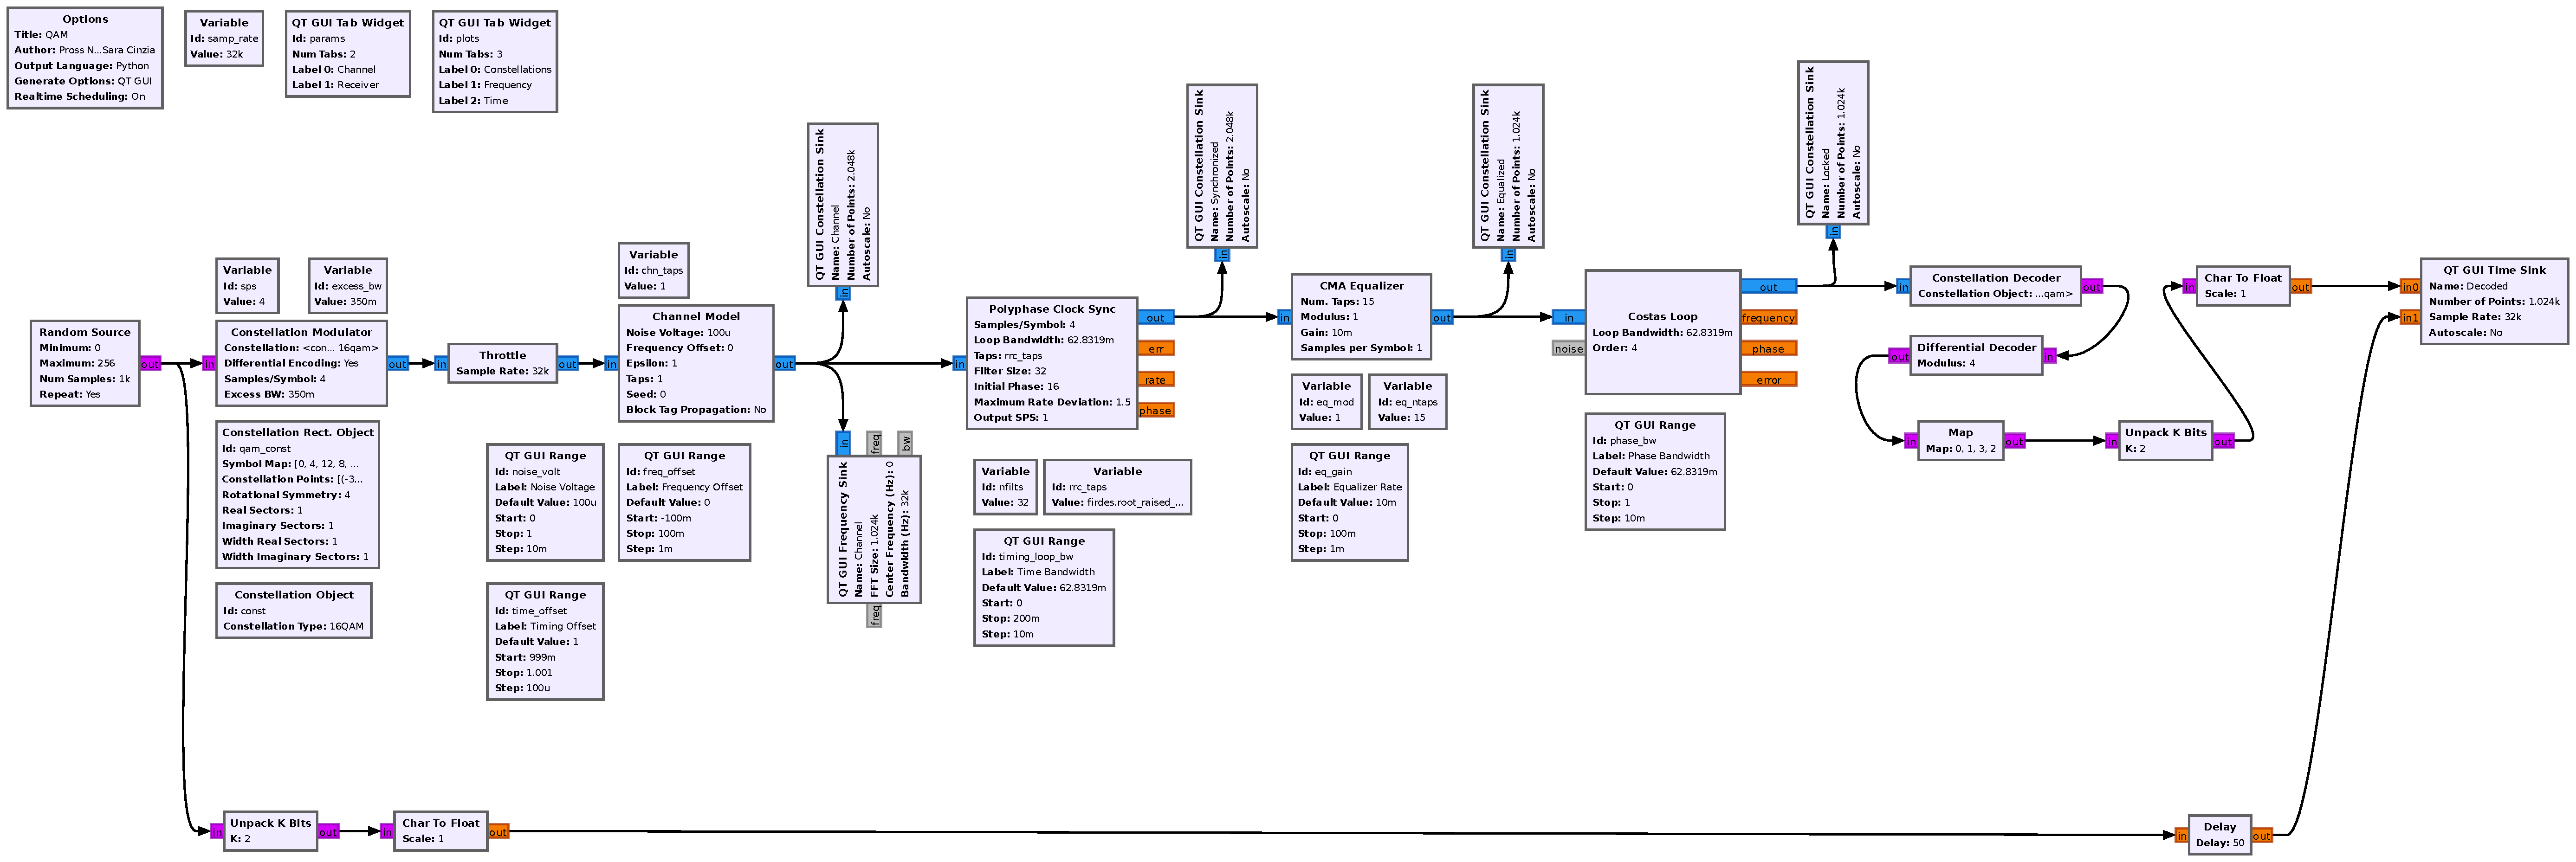
\includegraphics[width=\linewidth]{./figures/pdfs/qam_nogui.pdf}
	\caption{GNU Radio Blocks}
	\label{fig:simul16QAM_block}	
\end{figure}

\begin{figure}
	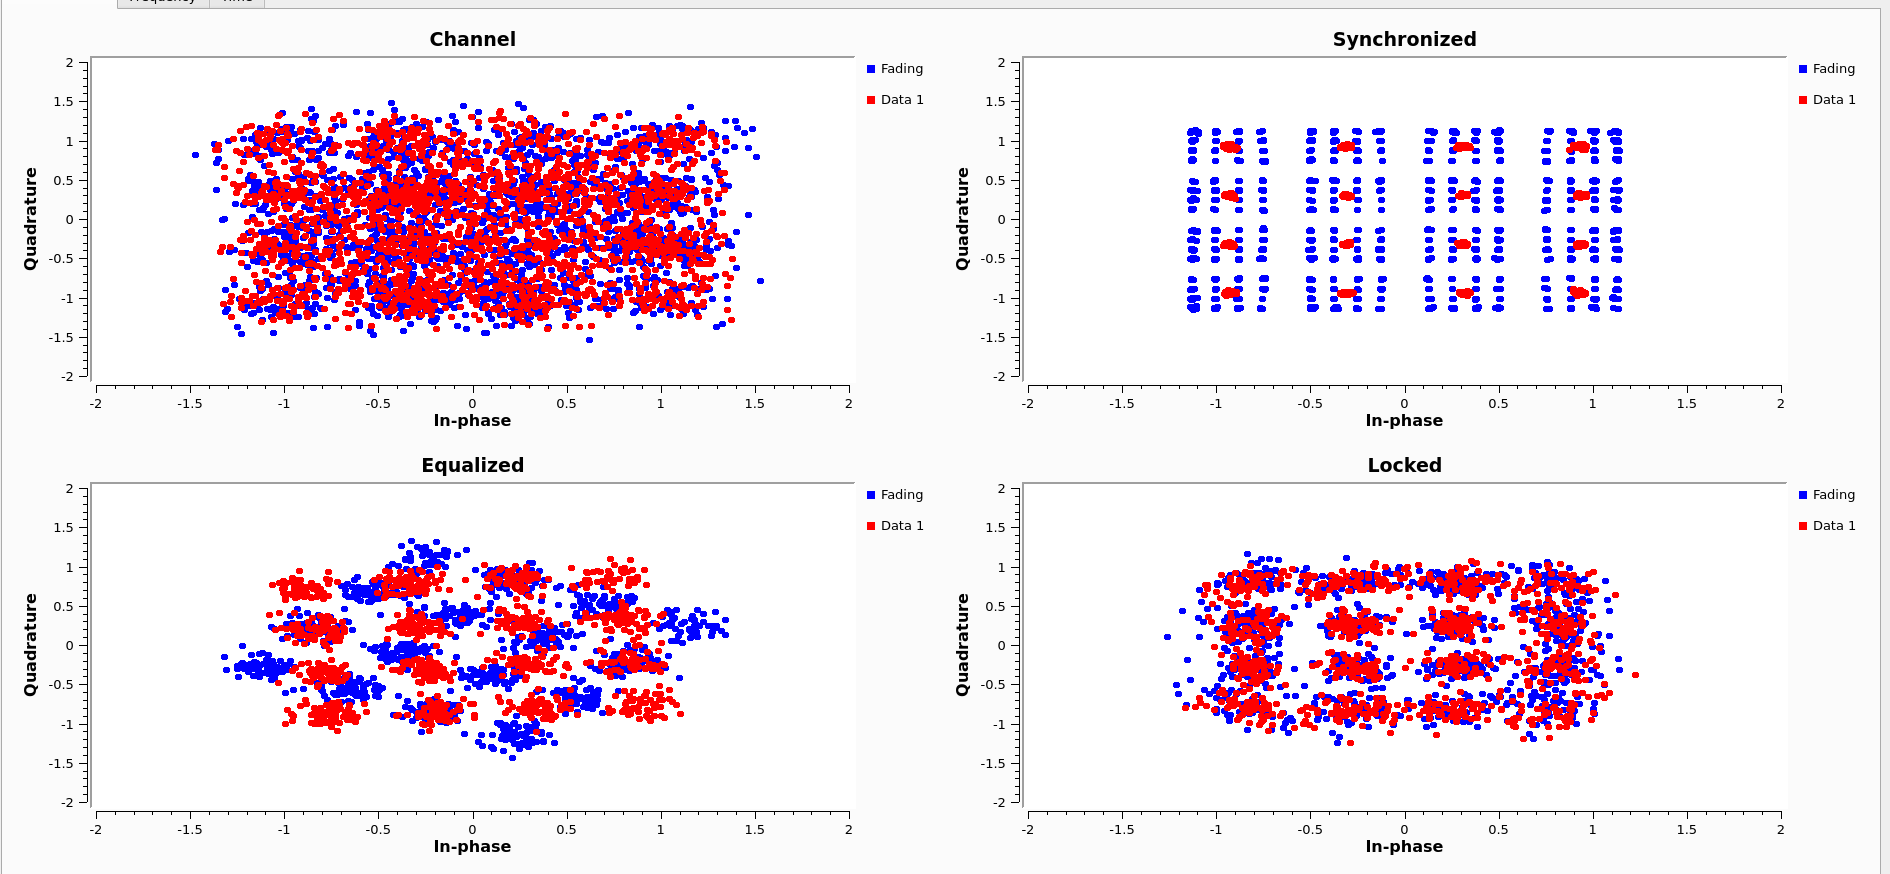
\includegraphics[width=\linewidth]{./figures/screenshots/QAM16_Fading_2.png}
	\caption{Simulation results}
	\label{fig:simul16QAM}	
\end{figure}

\begin{figure}
	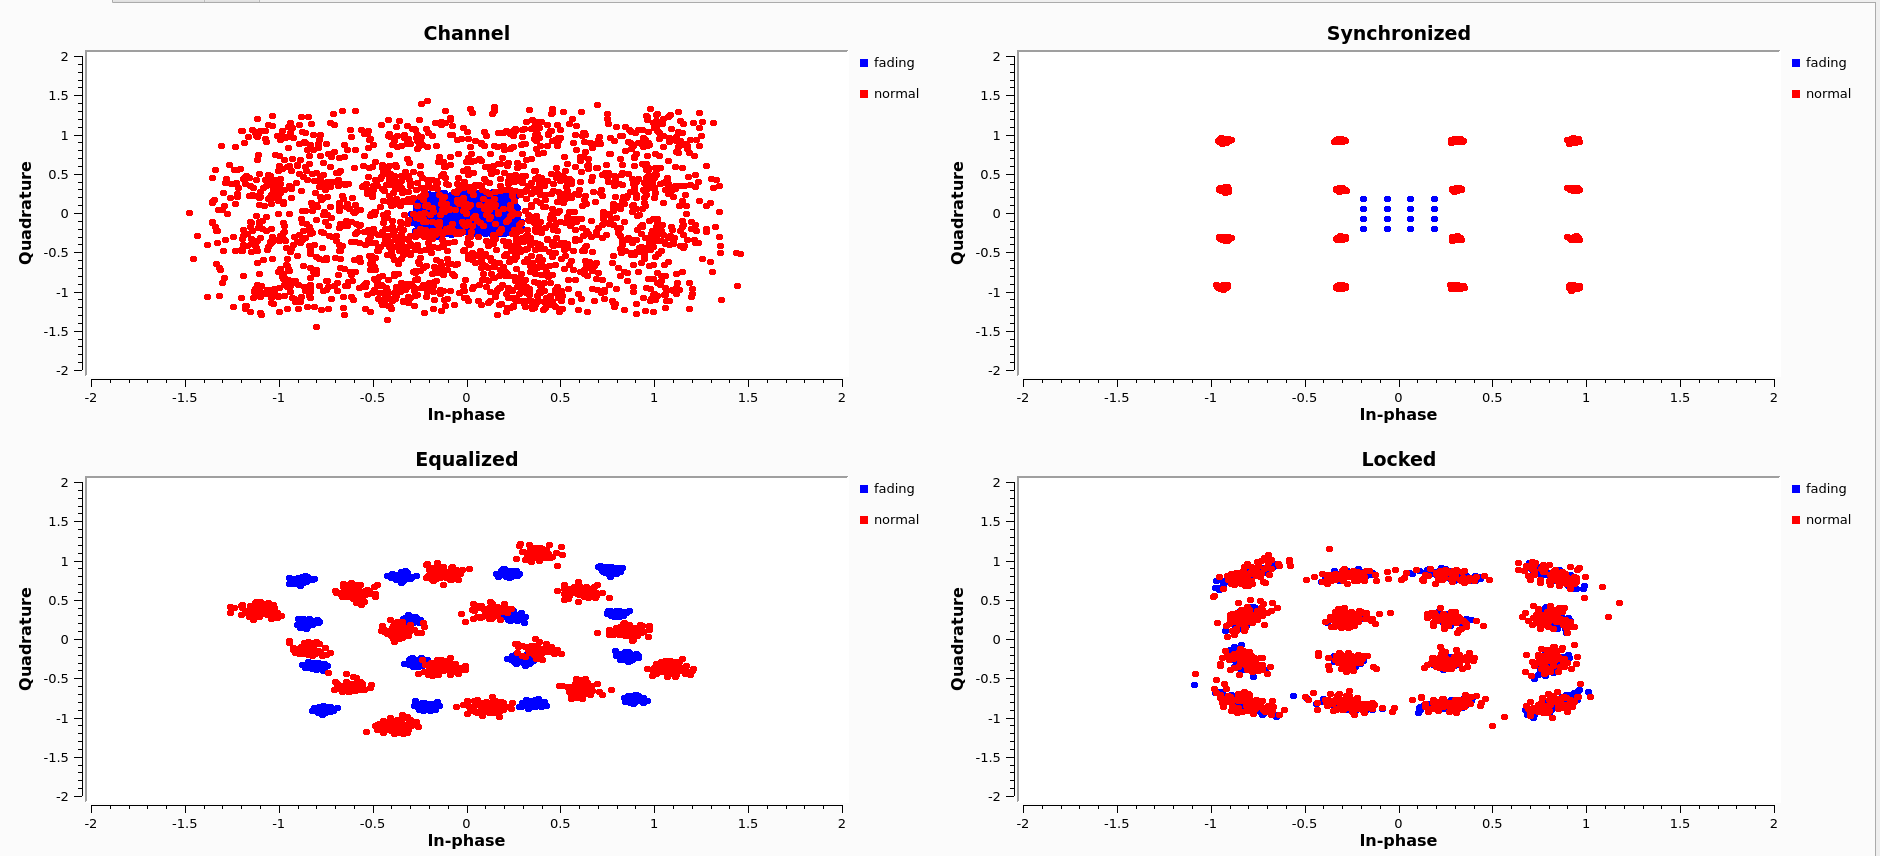
\includegraphics[width=\linewidth]{./figures/screenshots/QAM16_Fading_2_.png}
	\caption{Simulation results}
	\label{fig:simul16QAM_1}	
\end{figure}

\begin{table}[]
	\centering
	\caption{Modulation settings for different scheme}
	\begin{tabular}{ccc}
		\toprule
		Modulation Scheme & Samples per Symbol & Costas Loop Order\\
		\midrule
		BPSK  & 1 & 2 \\
		QPSK  & 2 & 4 \\
		8PSK  & 3 & 8 \\
		16QAM & 4 & 4 \\
		\bottomrule
	\end{tabular}
	\label{tab:modulation_settings}
\end{table}

\begin{figure}
	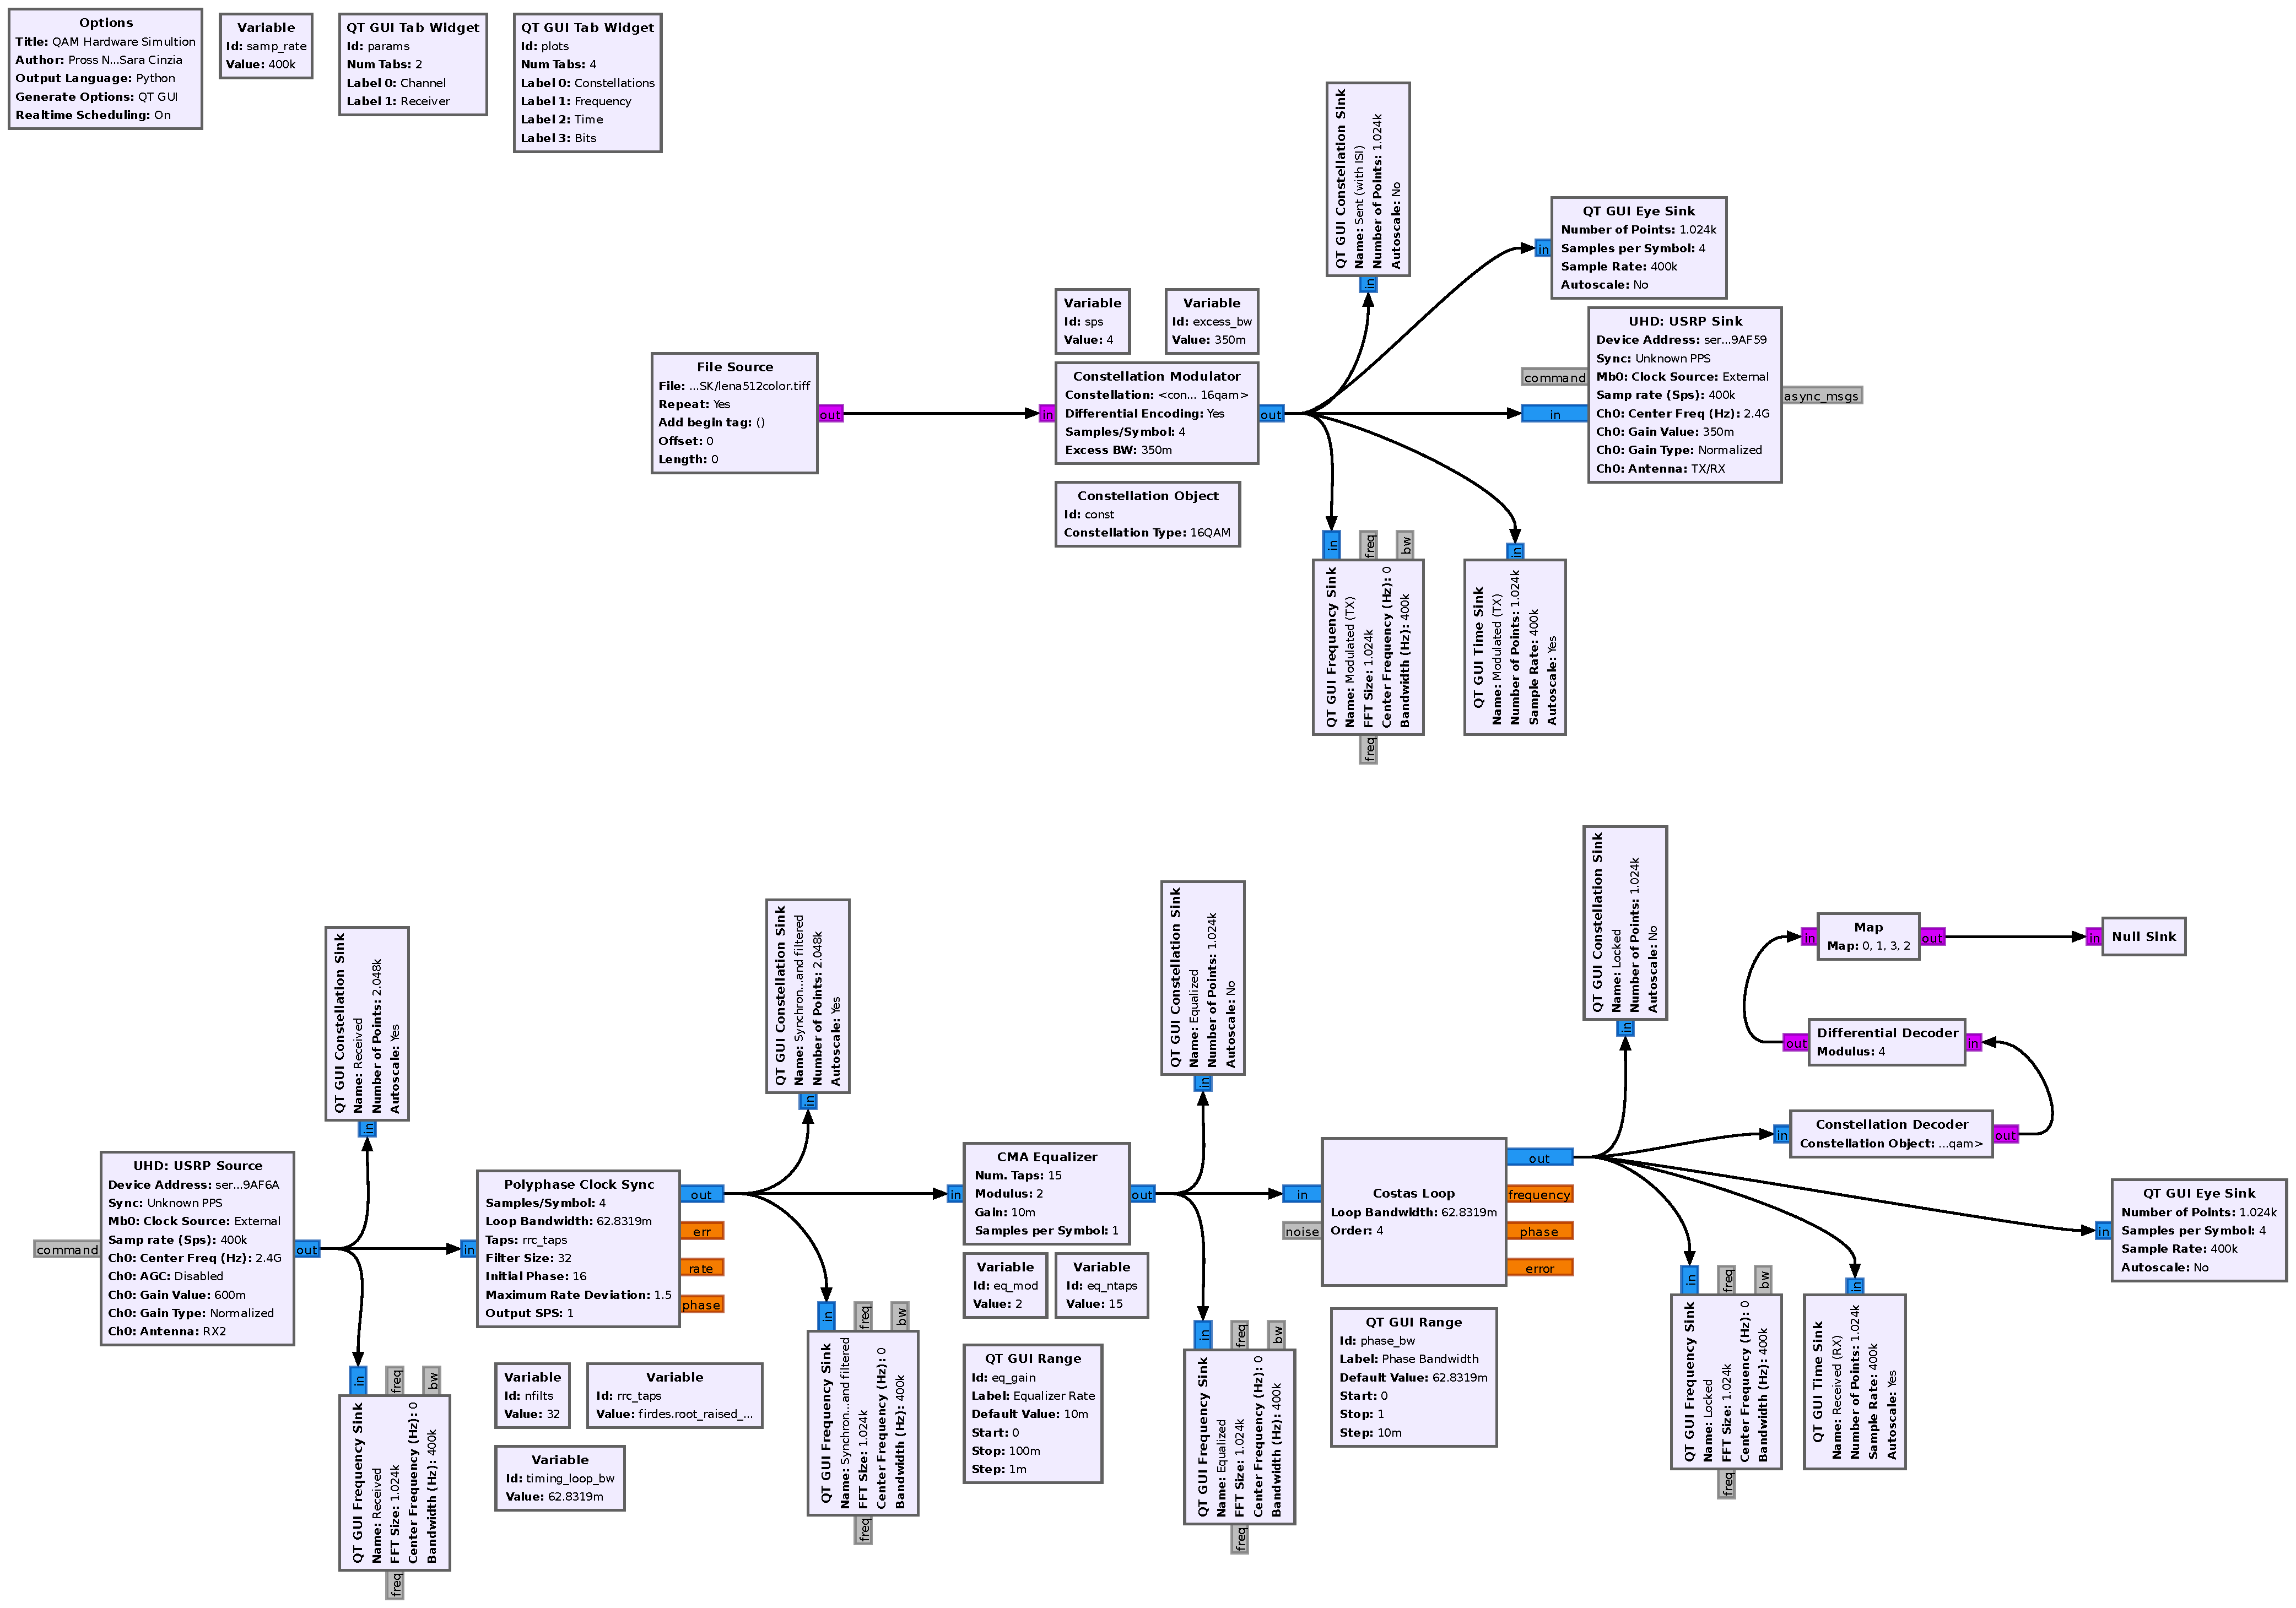
\includegraphics[width=\linewidth]{./figures/pdfs/qam_Hardware_1711.pdf}
	\caption{GNU Radio Blocks Hardware}
	\label{fig:simul16QAM_Hardware_Aufbau}	
\end{figure}

\begin{figure}
	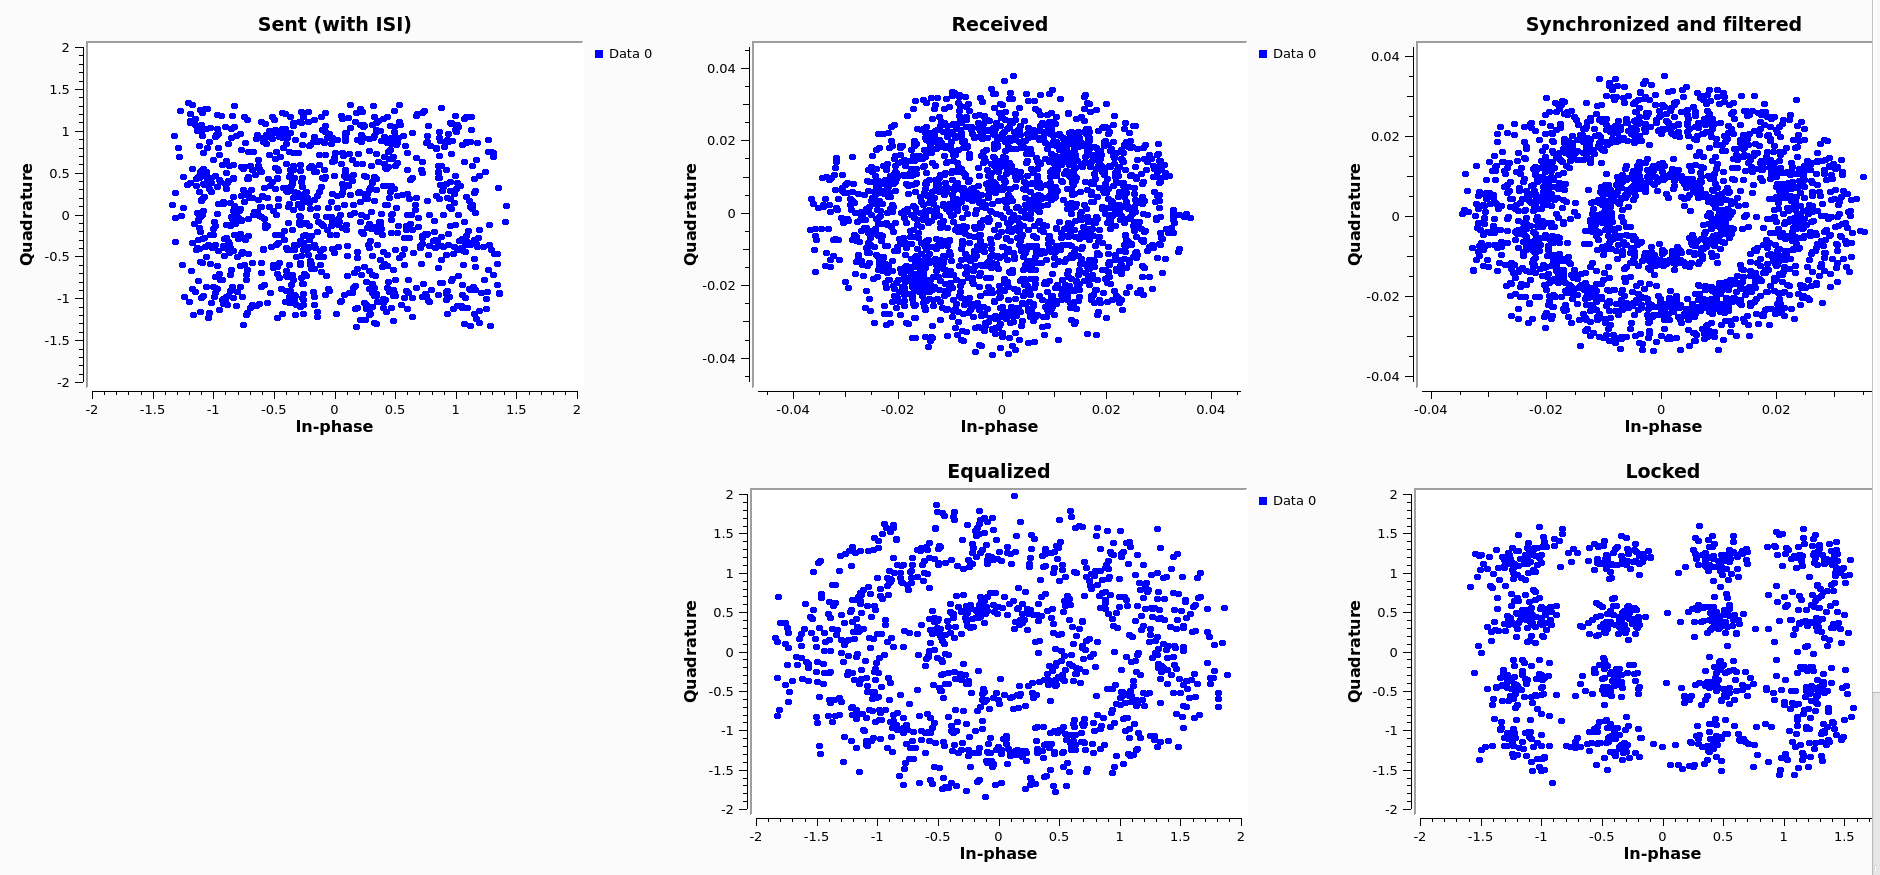
\includegraphics[width=\linewidth]{./figures/screenshots/QAM16_Hardware_1711.png}
	\caption{Hardware results}
	\label{fig:simul16QAM__Hardware}	
\end{figure}

% To Do: Picture of the setup

\begin{table}[]
	%To DO sepzifikationen ampssen / genauer? https://www.ettus.com/wp-content/uploads/2019/01/b200-b210_spec_sheet.pdf
	%https://kb.ettus.com/B200/B210/B200mini/B205mini#FAQ
	\centering
	\caption{USRP B210 specifications}
	\begin{tabular}{ll}
		\toprule
		Dimensions               & \(9.7 \times 15.5 \times 1.5\) cm \\
		Ports                    & 2 TX, 2 RX, Half or Full Duplex     \\
		RF frequencies           & from 70MHz to 6GHz                    \\
		Bandwidth                & 200kHz -- 56MHz                       \\
		External reference input & 10 MHz                                \\
		\bottomrule
	\end{tabular}
\label{tab:USRP B210 specifications}
\end{table}
